% Generated by tools/docx_tex.py from v1_2_base.docx. The .docx is the layout master;
% this file holds the text. Build the .docx with: docx_tex.py build <base.docx> <this.tex> <out.docx>
\documentclass[12pt]{article}
\usepackage{fontspec}\setmainfont{Liberation Serif}
\usepackage[russian]{babel}\usepackage[margin=2.5cm]{geometry}\usepackage{graphicx}
\begin{document}

% @p 0
УДК 621.3962.3.5. Математическое и программное обеспечение вычислительных систем, комплексов и компьютерных сетей

% @p 1
DOI

% @p 2
\subsection*{Подход к валидации автоматных спецификаций на основе перемножения вложенных автоматов}

% @p 3
В. А. Назарова, Бакалавр прикладной математики и информатики, orcid.org/0009-0000-0352-7885, nazarov.vladimir.a@gmail.comА. А. Шалыто, Докт. техн. наук, Профессор, orcid.org/0000-0002-2723-2077

% @p 4
аСанкт-Петербургский национальный исследовательский университет информационных технологий, механики и оптики, Кронверкский пр., 49, Санкт-Петербург, 197101, РФ

% @p 5
Введение: … Цель: … Методы: … Результаты: предлагаемый: … Практическая значимость: … Обсуждение: …

% @p 6
Ключевые слова – автоматы, вложенные автоматы, перемножение автоматов, валидация.

% @p 33
UDC 621.396

% @p 34
DOI

% @p 35
\subsection*{An approach to validating automaton specifications based on the product of nested automata}

% @p 36
V. A. Nazarova, Bachelor of science in applied mathematics and informatics, orcid.org/0009-0000-0352-7885, nazarov.vladimir.a@gmail.comA. A. Shalyto, Dr. Sc., Tech, Professor, orcid.org/0000-0002-2723-2077

% @p 37
aSaint Petersburg National Research University of Information Technologies, Mechanics and Optics, 49 Kronverksky Ave., 197101 St. Petersburg, Russian Federation

% @p 38
Introduction: ... Purpose: ... Methods: ... Results: ... Practical relevance: ... Discussion: ...

% @p 39
Keywords – automata, nested automata, automata composition, validation.

% @p 43
\subsection*{Введение}

% @p 44
% 1 контекст: что было сделано раньше.
% 2 связь: «новизна подхода» – уточняет, чем подход из 1 отличался.
% 3 связь: где подход показан (на какой системе).
% 4 связь: пример вложенности из 2 внутри системы из 3.
% 5 связь: «однако» – противопоставление: подход из 1 работал не всегда.
В предыдущей работе [x] был предложен подход к валидации автоматных спецификаций, основанный на перемножении автоматов. Новизна подхода состояла в перемножении вложенных автоматов – автоматов, размещенных в состояниях других автоматов. Подход был продемонстрирован на системе «игровой автомат» [x] из трёх взаимосвязанных автоматов: «Игровая машина» ($A_{0}$), «Монетоприемник» ($A_{1}$) и «Игровые барабаны» ($A_{2}$). В этой системе автомат $A_{2}$ вложен в состояние «Игра» автомата $A_{0}$. Однако у подхода было три ограничения:
% @comment: Круг 2. Текст переписан ради связности и простых слов: у каждого предложения явная связь с предыдущим, термины вводятся до использования. Смысл и термины соавтора сохранены. Связи по предложениям записаны в review/round2.py. Правки первого круга приняты; каждая видна в решённом примечании «Круг 1. Было: …».

\begin{enumerate}
% @p 45
\item В состояние мог быть вложен только один автомат.
% @p 46
\item Автомат мог быть вложен только в одно состояние.
% @p 47
\item Содержать вложенные автоматы мог только один из двух перемножаемых автоматов.
\end{enumerate}

% @p 48
% связь: ответ на ограничения из списка – «эти ограничения».
В настоящей работе предлагается метод валидации автоматных спецификаций на основе перемножения вложенных автоматов, в котором эти ограничения сняты.

% @p 49
\subsection*{Постановка задачи}

% @p 50
\subsection*{…}

% @p 51
\subsection*{Основные понятия и этапы подхода к валидации}

% @p 52
% 1 что получает автомат: три вида входных воздействий.
% 2 связь: раскрывает третий вид из 1 (запись условия).
% 3 связь: возвращается к первому виду из 1 и делит его на два вида.
% 4 связь: первый вид событий из 3, вводит термин «событие среды» (он нужен дальше).
% 5 связь: второй вид событий из 3.
% 6 связь: зачем нужны остальные виды из 1 – они входят в гварды.
% 7 связь: определение гварда из 6.
% 8 связь: после входов – выходы; третий вид выходов – это то, что проверяют
%   условия из 2 у других автоматов.
Входными воздействиями автомата в общем случае являются события e, входные переменные x и условия проверки состояний других автоматов. Условие проверки состояния записывается как yk = v (автомат k находится в состоянии v) или yk != v (автомат k не находится в состоянии v). События бывают двух видов. Событие среды поступает в систему автоматов извне, например при нажатии кнопки. Адресованное событие посылает один автомат другому: автомат-отправитель указывает его среди выходов на соответствующем переходе, а автомат-получатель принимает его только в момент этого перехода. Входные переменные и условия проверки состояний используются в гвардах. Гвардом называется условие на переходе – булева формула от входных воздействий; если гвард не выполнен, переход не срабатывает. Выходными воздействиями автомата являются события, выходные переменные z и условия проверки его состояний, которые используют другие автоматы.
% @comment: Круг 2. Открытый вопрос первого круга (A5) решён так: термин «событие среды» введён здесь явно, потому что он используется дальше. Запись «! – инверсия» заменена расшифровкой yk != v.

% @p 53
% 1 вводит термин «родительский» (нужен дальше).
% 2 связь: правило работы вложенного автомата через этот термин.
Автомат, в состояние которого вложен другой автомат, называется родительским. Вложенный автомат реагирует на события, только пока родительский автомат находится в этом состоянии.

% @p 54
% 1 возврат к подходу из введения: из чего он состоит.
% 2 связь: первая часть из 1.
% 3 связь: вторая часть из 1 и когда она нужна.
% 4 связь: те же части как последовательность этапов.
Подход к валидации, предложенный в предыдущей работе [x], состоит из двух частей. Первая часть – разработанный авторами метод перемножения автоматов, в том числе вложенных; он подробно изложен в той же работе. Вторая часть – ручная эвристическая корректировка перемножаемых автоматов; она нужна, если автомат-произведение получился громоздким. Подход состоит из следующих этапов, из которых этапы 1–4 составляют метод перемножения:

\begin{enumerate}
% @p 55
\item Выбор пары автоматов.
% @p 56
\item Построение начального состояния произведения из начальных состояний пары.
% @p 57
\item Построение множества вершин и рёбер произведения. Для очередного состояния определяются события, на которые может отреагировать хотя бы один из автоматов, с учётом вложенности и адресованных событий. Для каждого такого события проверяются гварды и строится переход в новое состояние произведения.
% @p 58
\item Формирование автомата-произведения из множества вершин и рёбер, построенного на предыдущем этапе.
% @p 59
% связь: «дедлок» объяснён в скобках простыми словами.
\item Визуальная валидация автомата-произведения: проверка его корректности, например отсутствия дедлоков (состояний, из которых нет выхода), и при необходимости эвристическая корректировка пары перемножаемых автоматов.
% @p 60
\item Для системы из более чем двух автоматов этапы 1–5 повторяются: произведение очередной пары умножается на следующий автомат.
% @p 61
% 1 что сравнивается; 2 связь: что делать, если сравнение не прошло.
\item Валидация (в инженерном смысле этого слова): автомат-произведение и исходная (откорректированная) система автоматов получают одинаковые входные воздействия, и их функционирование сравнивается. Если поведение различается, исходную систему автоматов корректируют и применяют подход повторно.
\end{enumerate}

% @p 62
% 1 связь: возврат к ограничениям из введения – что с ними сделано и что с этапами.
% 2 связь: какие именно этапы затронуты доработкой из 1.
% 3 связь: где доработки описаны и на каком примере.
Чтобы снять ограничения 1–3, метод перемножения доработан, но перечень этапов не изменился. Доработки касаются этапов 3 и 4: того, как проверяются гварды, ссылающиеся на состояния других автоматов, и как определяется, какие автоматы вложены в состояние произведения. Каждая доработка описана в разделе «Доработки метода» на примере системы автоматов, которая вводится в следующем разделе.

% @p 63
\subsection*{Дополненная система автоматов}

% @p 64
% 1 что было в предыдущей работе.
% 2 связь: «чтобы показать» – зачем добавлены новые автоматы.
% 3 связь: где видно, какой автомат что показывает.
В предыдущей работе система «игровой автомат» состояла из трёх автоматов: «Игровая машина» $A_{0}$ (рис. 1), «Монетоприемник» $A_{1}$ (рис. 2) и «Игровые барабаны» $A_{2}$ (рис. 3). Чтобы показать снятие ограничений, в неё добавлены два новых автомата: «Джекпот-счётчик» $A_{3}$ (рис. 4) и «Звуки» $A_{4}$ (рис. 5). В таблице 1 для каждого случая вложенности в полученной системе указано, снятие какого ограничения он демонстрирует.

% @p 66
Таблица 1. Случаи вложенности, демонстрирующие снятие ограничений

\begin{tabular}{|p{0.45\linewidth}|p{0.45\linewidth}|}
% @p 67
Ограничение &
% @p 68
Иллюстрация в системе \\ \hline
% @p 69
– &
% @p 70
Автомат $A_{2}$ вложен в состояние «Игра» автомата $A_{0}$ (случай предыдущей работы) \\ \hline
% @p 71
1 &
% @p 72
В состояние «Игра» автомата $A_{0}$ вложены автоматы $A_{2}$, $A_{3}$ и $A_{4}$ \\ \hline
% @p 73
2 &
% @p 74
Автомат $A_{4}$ вложен в три состояния: «Игра» и «Выдача жетона» автомата $A_{0}$, «Выплата джекпота» автомата $A_{3}$ \\ \hline
% @p 75
3 &
% @p 76
Автомат $A_{4}$ вложен в состояние «Выплата джекпота» автомата $A_{3}$, который сам вложен в состояние «Игра» автомата $A_{0}$ \\ \hline
\end{tabular}

% @p 85
\subsection*{Автомат 1. «Игровая машина» ($A_{0}$)}

% @img 86
\begin{center}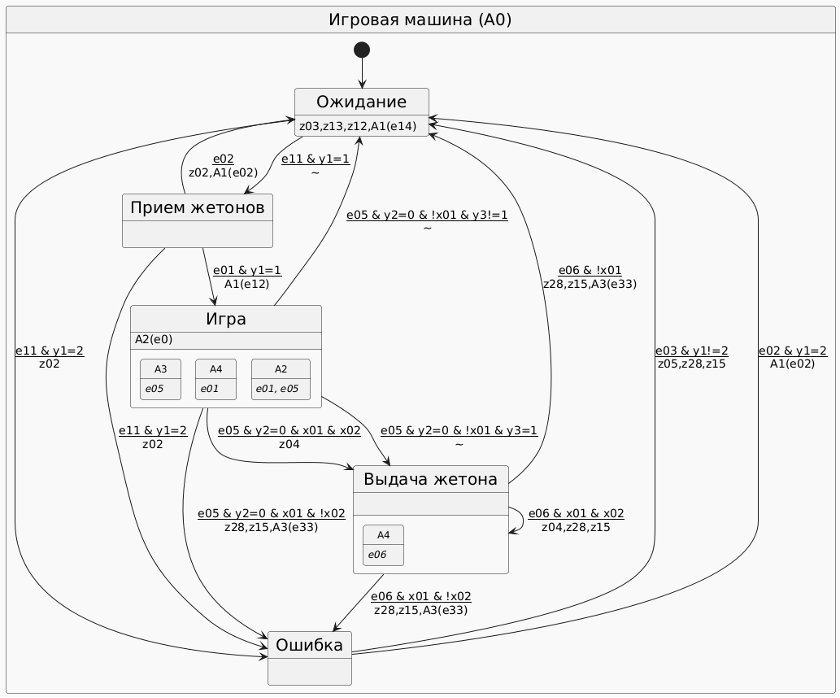
\includegraphics[width=0.8\linewidth]{media/image1.png}\end{center}
% @p 87
Рис. 1. Диаграмма состояний автомата $A_{0}$. В состояние «Игра» вложены автоматы $A_{2}$, $A_{3}$ и $A_{4}$, в состояние «Выдача жетона» – автомат $A_{4}$

% @p 100
Таблица 2. Входные и выходные воздействия автомата «Игровая машина» ($A_{0}$)

% @img 101
\begin{center}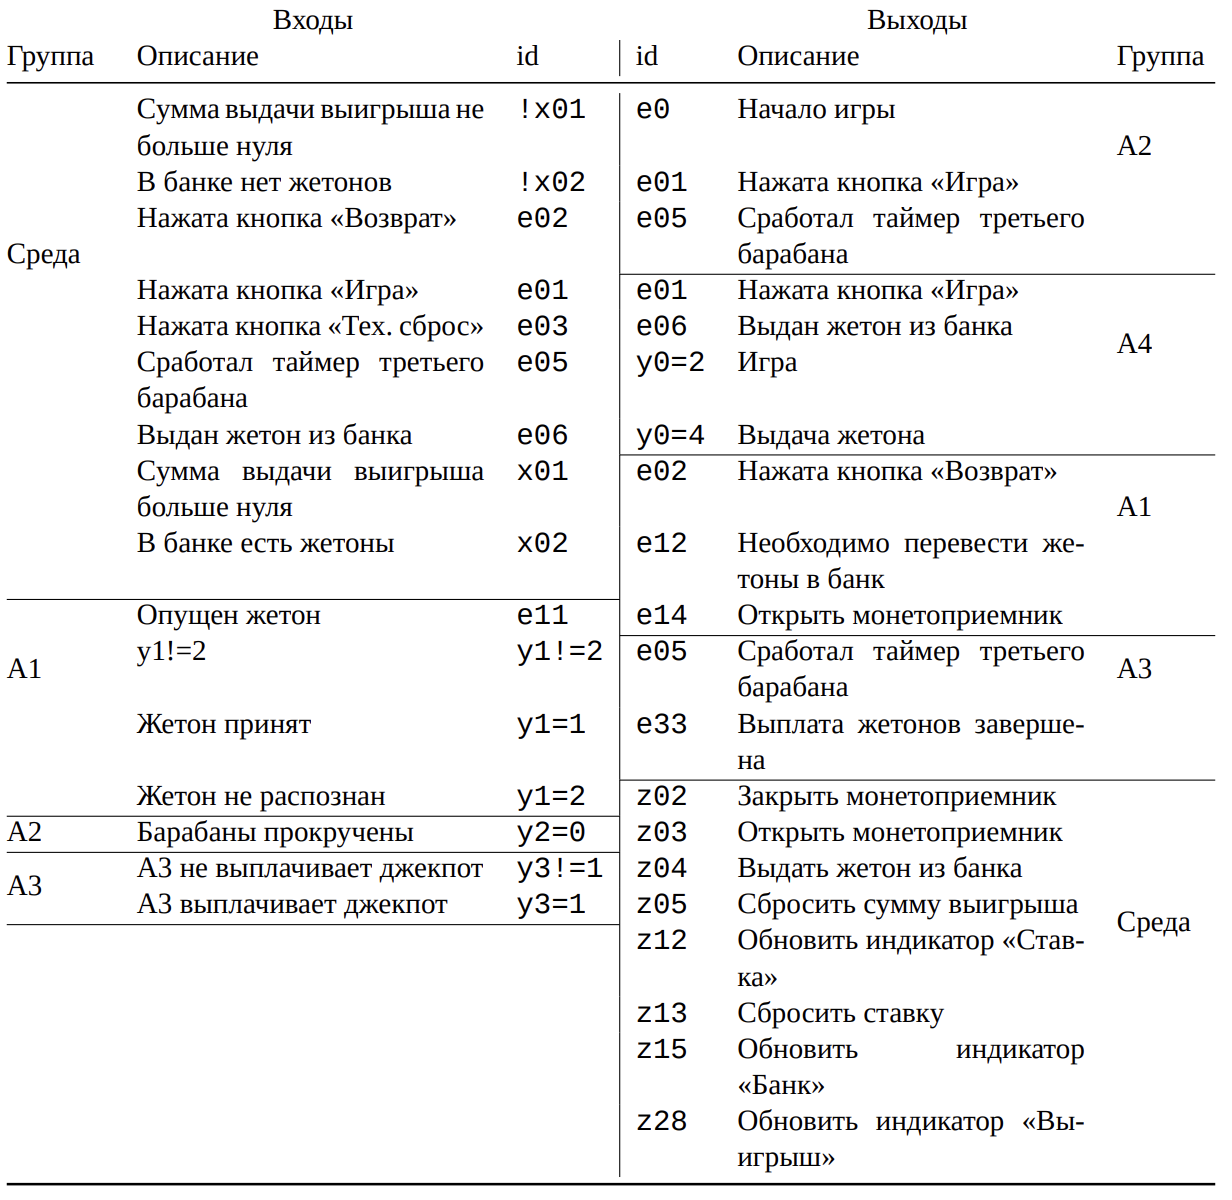
\includegraphics[width=0.8\linewidth]{media/image12.png}\end{center}
% @p 112
\subsection*{Автомат 2. «Монетоприемник» ($A_{1}$)}

% @img 113
\begin{center}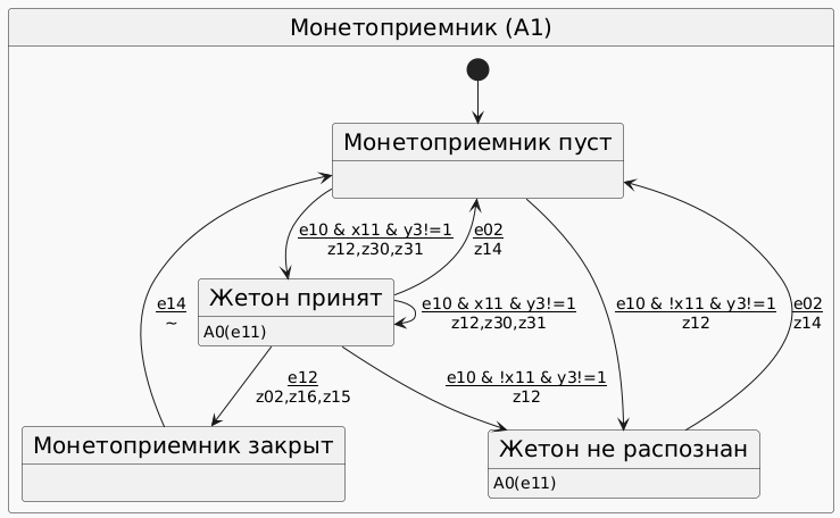
\includegraphics[width=0.8\linewidth]{media/image8.png}\end{center}
% @p 114
Рис. 2. Диаграмма состояний автомата $A_{1}$

% @p 116
Таблица 3. Входные и выходные воздействия автомата «Монетоприемник» ($A_{1}$)

% @img 117
\begin{center}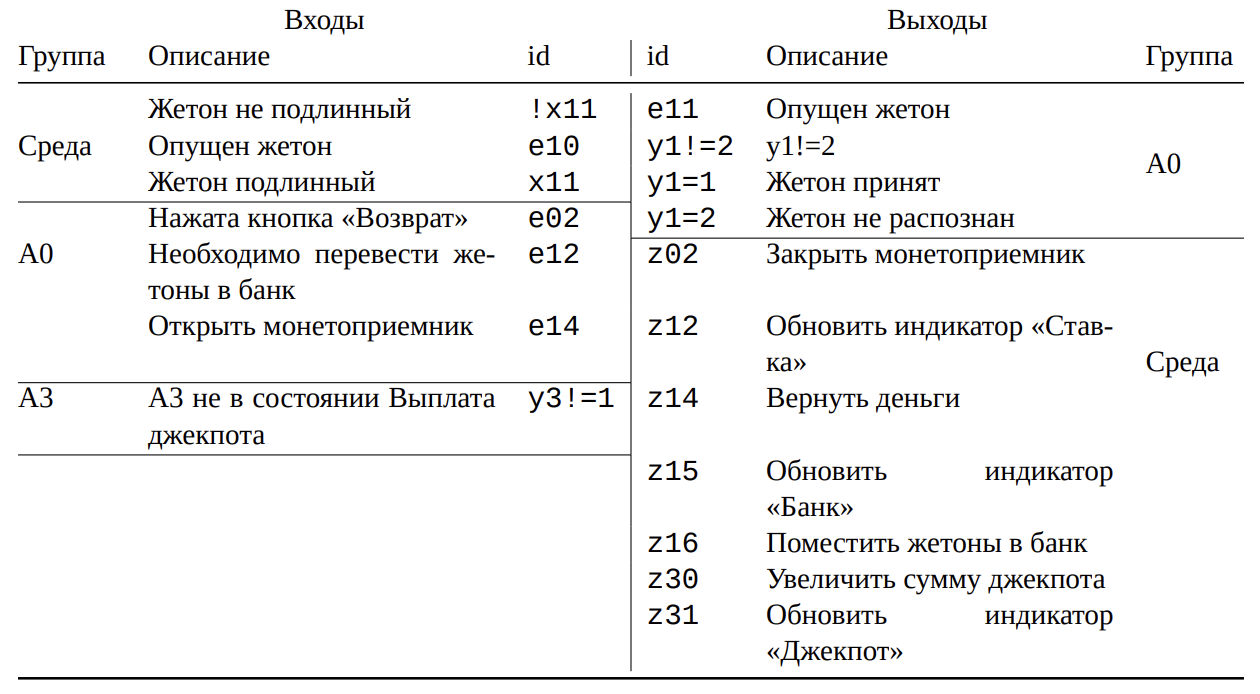
\includegraphics[width=0.8\linewidth]{media/image11.png}\end{center}
% @p 123
\subsection*{Автомат 3. «Игровые барабаны» ($A_{2}$)}

% @img 124
\begin{center}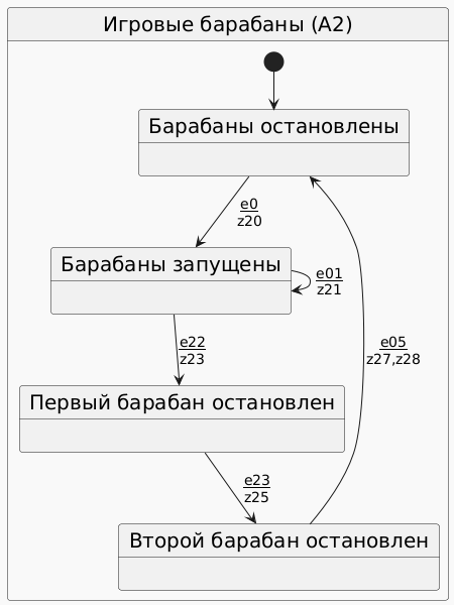
\includegraphics[width=0.8\linewidth]{media/image5.png}\end{center}
% @p 125
Рис. 3. Диаграмма состояний автомата $A_{2}$

% @p 127
Таблица 4. Входные и выходные воздействия автомата «Игровые барабаны» ($A_{2}$)

% @img 128
\begin{center}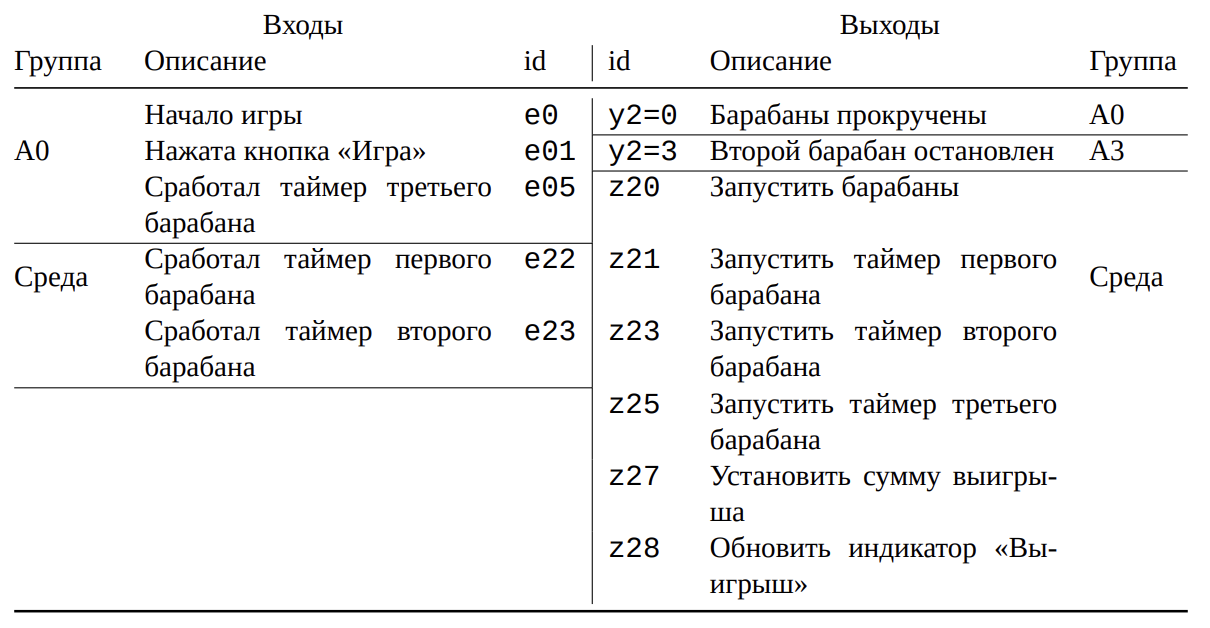
\includegraphics[width=0.8\linewidth]{media/image10.png}\end{center}
% @p 131
\subsection*{Автомат 4. «Джекпот-счётчик» ($A_{3}$)}

% @img 132
\begin{center}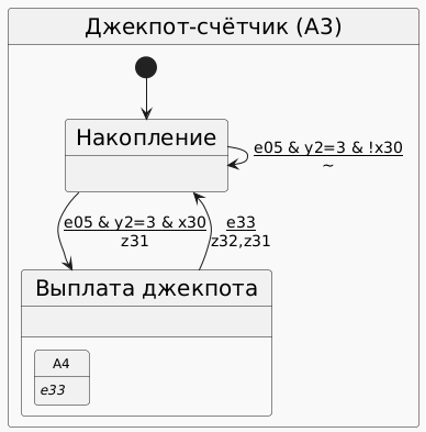
\includegraphics[width=0.8\linewidth]{media/image2.png}\end{center}
% @p 133
Рис. 4. Диаграмма состояний автомата $A_{3}$. В состояние «Выплата джекпота» вложен автомат $A_{4}$; сам автомат $A_{3}$ вложен в состояние «Игра» автомата $A_{0}$

% @p 135
Таблица 5. Входные и выходные воздействия автомата «Джекпот-счётчик» ($A_{3}$)

% @img 136
\begin{center}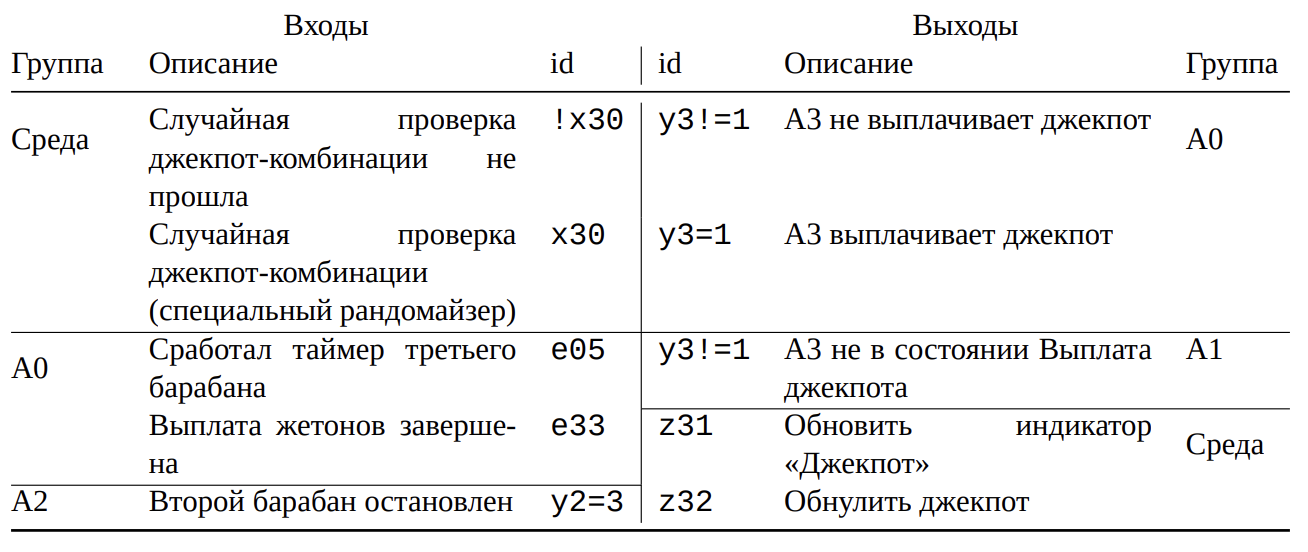
\includegraphics[width=0.8\linewidth]{media/image7.png}\end{center}
% @p 137
% 1 что будет показано (тезис раздела).
% 2 связь: первый довод – вложенность A3 вместе с A2 (ограничение 1).
% 3 связь: что общего у A2 и A3 из 2 – общее событие.
% 4 связь: как A3 переходит в новое состояние после этого события.
% 5 связь: что значит первое условие из 4.
% 6 связь: как A3 выходит из состояния, в которое вошёл в 4.
% 7 связь: тот же e33 из 6 получает A4 – мост к следующему автомату.
Покажем на автоматах $A_{3}$ и $A_{4}$, что в расширенной системе ограничения 1–3 отсутствуют. Автомат $A_{3}$ вложен в состояние «Игра» автомата $A_{0}$ вместе с автоматом $A_{2}$, то есть в одно состояние вложено несколько автоматов (снятие ограничения 1). Оба автомата реагируют на одно и то же событие среды e05 («Сработал таймер третьего барабана»). По этому событию автомат $A_{3}$ переходит в состояние «Выплата джекпота», если выполнен гвард из двух условий: y2=3 (второй барабан остановлен) и x30 (случайная проверка джекпот-комбинации прошла). Первое условие показывает, что автомат $A_{3}$ использует состояние автомата $A_{2}$, вложенного в то же состояние. Из состояния «Выплата джекпота» автомат $A_{3}$ выходит по событию e33, которое ему адресует автомат $A_{0}$ после выдачи жетонов; при этом джекпот обнуляется. Это же событие через вложенность получает и автомат $A_{4}$.

% @p 138
\subsection*{Автомат 5. «Звуки» ($A_{4}$)}

% @img 139
\begin{center}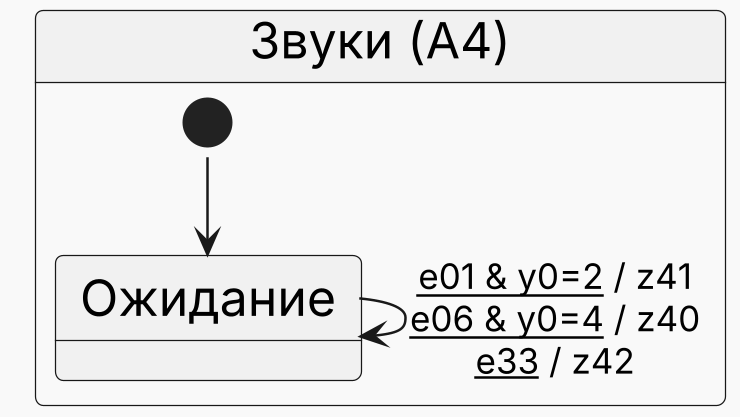
\includegraphics[width=0.8\linewidth]{media/fig5_a4.png}\end{center}
% @p 140
Рис. 5. Диаграмма состояний автомата $A_{4}$: одно состояние и петля с тремя пометками, по одной на каждое место вложения
% @comment: Рисунок заменён: три перехода-петли на одной стрелке слились в одну пометку и читались как один переход. Теперь каждый переход – отдельная строка вида «условие / действие».

% @p 142
Таблица 6. Входные и выходные воздействия автомата «Звуки» ($A_{4}$)

% @img 143
\begin{center}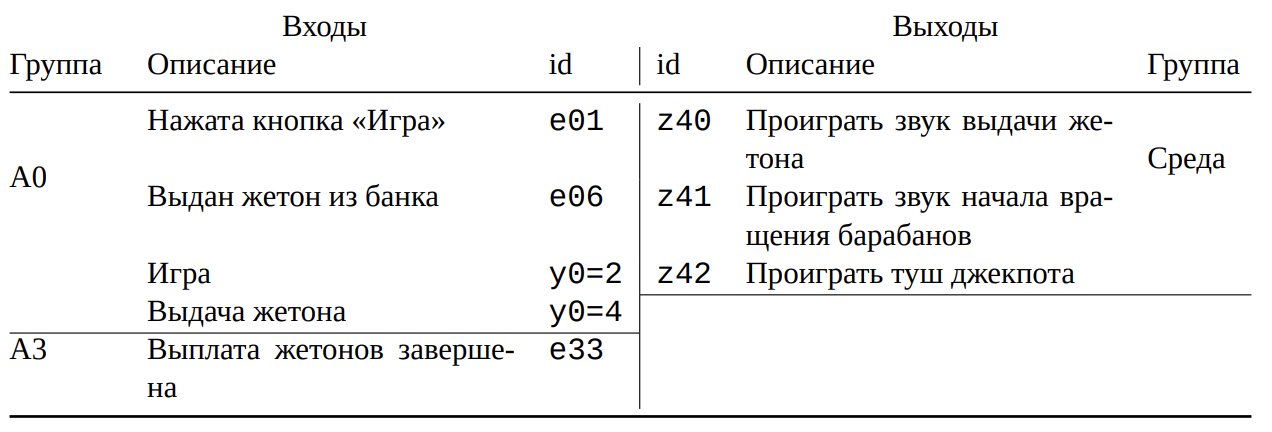
\includegraphics[width=0.8\linewidth]{media/image6.png}\end{center}
% @p 144
% 1 тезис для A4; 2 связь: раскрывает тезис по ограничениям.
Автомат $A_{4}$ демонстрирует снятие ограничений 2 и 3. Он вложен в три состояния (снятие ограничения 2), и одно из них принадлежит автомату $A_{3}$, который сам вложен в автомат $A_{0}$ (снятие ограничения 3).

% @p 145
% 1 первые два самоперехода и их события.
% 2 связь: как метод определяет, может ли A4 реагировать.
% 3 связь: «поэтому» – к чему это привело бы.
% 4 связь: «чтобы этого не было» – как это исключено.
Два самоперехода автомата $A_{4}$ – по событиям e01 (нажатие кнопки «Игра») и e06 (выдача жетона) – вызываются событиями среды, на которые реагирует и автомат $A_{0}$. Метод проверяет только, вложен ли автомат $A_{4}$ в текущее состояние автомата-произведения, но не различает, через какое из мест вложения. Поэтому без дополнительных условий автомат $A_{4}$ реагировал бы на e06 и в состоянии «Игра», где автомат $A_{0}$ на это событие не реагирует. Чтобы этого не было, самопереходы проверяют условия y0=2 и y0=4: реакция на e01 возможна только в состоянии «Игра» автомата $A_{0}$, а реакция на e06 – только в состоянии «Выдача жетона».

% @p 146
% 1 «третий» – продолжение после двух самопереходов.
% 2 связь: почему условие не нужно – откуда приходит e33.
% 3 связь: «поэтому» – когда именно A4 реагирует.
Третий самопереход – по событию e33 – дополнительного условия не требует. Событие e33 адресовано автоматом $A_{0}$ автомату $A_{3}$, а автомат $A_{4}$ получает его через вложенность, только когда автомат $A_{3}$ находится в состоянии «Выплата джекпота». Поэтому автомат $A_{4}$ реагирует на e33 одновременно с переходом, которым автомат $A_{3}$ выходит из этого состояния (см. доработку 4 в разделе «Доработки метода»).

% @p 148
\subsection*{Доработки метода}

% @p 149
\subsection*{Доработка 1}

% @p 150
Было. Гвард, который ссылается на состояние другого автомата, проверялся по номеру состояния этого автомата в автомате-произведении, полученном на предыдущих шагах перемножения.

% @p 151
% 1 что происходит при перемножении; 2 связь: «поэтому» – следствие для гвардов;
% 3 связь: «из-за этого» – следствие для ограничения 1; 4 связь: та же причина – ограничение 2.
Что ограничивало. При перемножении два состояния объединяются в одно, и номер состояния произведения перестаёт однозначно указывать состояние каждого исходного автомата. Поэтому гвард, ссылающийся на автомат, который уже вошёл в произведение, нельзя было проверить корректно. Из-за этого в состояние можно было вложить только один автомат (ограничение 1): при двух вложенных автоматах гварды, которые различают их состояния, переставали работать. По той же причине автомат нельзя было вложить больше чем в одно состояние (ограничение 2).

% @p 152
% 1 что хранится теперь; 2 связь: почему это не теряется; 3 связь: как это используется и что даёт.
Как исправили. Теперь для каждого состояния произведения хранится, в каком собственном состоянии находится каждый вошедший в него автомат. При объединении состояний эти сведения объединяются, поэтому они не теряются при перемножении цепочки автоматов. Гвард проверяется по этим сведениям и работает при любом числе автоматов, вложенных в одно состояние (ограничение 1), и при любом числе состояний, в которые вложен один автомат (ограничение 2).

% @p 153
\subsection*{Доработка 2}

% @p 154
% 1 что хранится в состоянии произведения (вводит «список вложенных автоматов»);
% 2 связь: как этот список составлялся.
Было. Каждое состояние произведения хранит список автоматов, вложенных в него, то есть тех, которые в этом состоянии реагируют на события. Для нового состояния этот список составлялся просто: списки двух перемножаемых автоматов объединялись.

% @p 155
% 1 связь: оценка способа из «Было» – когда он верен;
% 2 связь: «если же» – когда перестаёт быть верным;
% 3 связь: «рассмотрим» – конкретная цепочка для случая из 2;
% 4 связь: что должно выполняться для A4 из цепочки 3 и почему (два условия);
% 5 связь: какое из условий 4 проверял прежний способ;
% 6 связь: «поэтому» – к чему приводила потеря второго условия.
Что ограничивало. Такой способ верен, пока вложенные автоматы есть только у одного из двух перемножаемых автоматов (ограничение 3). Если же вложенный автомат сам содержит вложенный автомат, способ даёт ошибку. Рассмотрим цепочку из системы: автомат $A_{3}$ вложен в состояние «Игра» автомата $A_{0}$, а автомат $A_{4}$ вложен в состояние «Выплата джекпота» автомата $A_{3}$. Через это вложение автомат $A_{4}$ должен реагировать на события, только когда выполнены два условия: автомат $A_{3}$ находится в состоянии «Выплата джекпота», а автомат $A_{0}$ – в состоянии «Игра», потому что иначе не реагирует сам автомат $A_{3}$. Простое объединение списков проверяло только первое условие. Поэтому автомат $A_{4}$ считался вложенным при любом состоянии автомата $A_{0}$, если автомат $A_{3}$ оставался в состоянии «Выплата джекпота».

% @p 156
% 1 новое правило в общем виде; 2 связь: то же правило на примере из «Что ограничивало»;
% 3 связь: что остаётся как раньше.
Как исправили. Теперь список вложенного автомата добавляется в состояние произведения, только когда этот автомат сам может реагировать, то есть его родительский автомат находится в состоянии, в которое он вложен. В примере автомат $A_{4}$ попадает в список, только если автомат $A_{3}$ находится в состоянии «Выплата джекпота», а автомат $A_{0}$ – в состоянии «Игра». Если перемножаемые автоматы не вложены друг в друга, их списки, как и раньше, просто объединяются.

% @p 157
\subsection*{Доработка 3}

% @p 158
Было. Если автомат вложен в текущее состояние, на этапе 3 любое адресованное ему событие считалось способным само по себе вызвать переход в автомате-произведении, так же, как событие среды.

% @p 159
% 1 факт об адресованном событии; 2 связь: «поэтому» – к чему вело правило из «Было»;
% 3 связь: где это проявилось.
Что ограничивало. Адресованное событие возникает только в момент перехода автомата-отправителя. Поэтому, рассматривая его отдельно от этого перехода, метод строил переходы, которых нет в исходной системе. В рассматриваемой системе это проявилось при вложении автомата $A_{4}$ в автомат $A_{3}$ (ограничение 3): в автомате-произведении был переход, в котором автомат $A_{4}$ воспроизводил звуковой сигнал выигрыша джекпота (z42), а автомат $A_{3}$ оставался в состоянии «Выплата джекпота».

% @p 160
% 1 новое правило для событий среды; 2 связь: и для адресованных событий.
Как исправили. Теперь вложенный автомат реагирует на событие сам по себе, только если хотя бы один из автоматов, уже вошедших в произведение, объявляет это событие событием среды. Адресованное событие вложенный автомат получает только вместе с переходом автомата-отправителя.

% @p 161
\subsection*{Доработка 4}

% @p 162
Было. Адресованное событие поступало только автомату-получателю.

% @p 163
% 1 связь: «поэтому» – следствие из «Было»; 2 связь: пример в системе.
Что ограничивало. Поэтому автомат, вложенный в состояние получателя, не мог отреагировать на такое событие. В рассматриваемой системе автомат $A_{4}$ вложен в состояние «Выплата джекпота» автомата $A_{3}$, но не мог отреагировать на событие e33, по которому автомат $A_{3}$ выходит из этого состояния.

% @p 164
% 1 новое правило; 2 связь: где оказываются реакции; 3 связь: особый случай;
% 4 связь: «тогда» – как он обрабатывается; 5 связь: то же правило при сравнении на этапе 7.
Как исправили. Теперь адресованное событие получает не только получатель, но и автоматы, вложенные в то состояние, в котором получатель был до перехода. Их реакции входят в тот же переход автомата-произведения. Бывает, что такой вложенный автомат ещё не вошёл в произведение. Тогда переход произведения запоминает недоставленное событие и доставляет его, когда автомат войдёт в произведение. Так же события доставляются и при выполнении исходной (при необходимости откорректированной) системы автоматов, с которой автомат-произведение сравнивается на этапе 7.

% @p 165
\subsection*{Замечание о порядке умножения}

% @p 166
% 1 тезис: порядок важен в двух случаях; 2 связь: первый случай; 3 связь: «иначе» – что будет;
% 4 связь: пример.
Порядок, в котором перемножаются автоматы, важен в двух случаях. Первый случай – гварды: если гвард автомата Y ссылается на состояние автомата X, то автомат X должен войти в произведение не позднее автомата Y. Иначе результат умножения может не совпадать с поведением исходной системы. Например, так происходит при порядке $A_{0}$, $A_{2}$, $A_{1}$, потому что автомат $A_{0}$ содержит гвард на состояние автомата $A_{1}$.

% @p 167
% 1 переход к адресованным событиям: зависит от способа доставки; 2 связь: напрямую – не важен, почему;
% 3 связь: что изменилось.
Для адресованных событий требование зависит от того, как событие доставляется. Если получатель получает событие напрямую, порядок не важен. Раньше, если отправитель ещё не вошёл в произведение, получатель реагировал на его событие так, будто оно может возникнуть в любой момент, и появлялись лишние состояния. Теперь получатель не реагирует на такое событие, пока отправитель не войдёт в произведение.

% @p 168
% 1 второй случай из тезиса; 2 связь: «иначе» – что будет; 3 связь: «поэтому» – следствие для системы.
Второй случай, когда порядок важен, – события, которые приходят через вложенность (доработка 4): вложенный автомат должен войти в произведение после родительского. Иначе в момент доставки события родительскому автомату вложенный автомат уже входит в произведение, переход не запоминает недоставленное событие, и реакция вложенного автомата теряется. Поэтому в рассматриваемой системе автомат $A_{4}$ умножается после автомата $A_{3}$, а при порядке $A_{0}$, $A_{1}$, $A_{2}$, $A_{4}$, $A_{3}$ программа сообщает об ошибке.

% @p 169
Как снять оба требования и какие порядки перемножения допустимы в общем случае, остаётся предметом дальнейшей работы.

% @p 170
\subsection*{Замечание об обратном вызове}

% @p 171
% 1 тезис; 2 связь: определение термина из 1; 3 связь: что делает метод в этом случае;
% 4 связь: как это обнаруживается.
Как и в предыдущей работе [x], обратный вызов не допускается. Обратный вызов – это случай, когда автомат A на своём переходе адресует событие автомату B, а автомат B в ответ адресует событие автомату A. Метод такую ответную реакцию не строит: в автомате-произведении автомат A на неё не реагирует. Расхождение с исходной системой при этом обнаруживается на этапе 7, что проверено на паре автоматов с обратным вызовом.

% @p 172
\subsection*{Замечание о моменте первой реакции вложенного автомата}

% @p 173
% 1 правило; 2 связь: «поэтому» – следствие; 3 связь: как обойти; 4 связь: пример обхода;
% 5 связь: что нужно для снятия; 6 связь: оценка сложности.
Вложенность проверяется по состоянию родительского автомата до перехода. Поэтому автомат, вложенный в целевое состояние перехода, не реагирует на событие, которое вызвало этот переход: он начинает реагировать только на следующие события. Если реакция нужна сразу при входе в состояние, её передают адресованным событием. Так, автомат $A_{0}$ при входе в состояние «Игра» адресует автомату $A_{2}$ событие e0 («Начало игры»). Чтобы снять это ограничение, метод должен при построении перехода опрашивать автоматы, вложенные в его целевое состояние, хотя это состояние в автомате-произведении ещё не построено. Это требует существенно изменить устройство метода и остаётся предметом дальнейшей работы.

% @p 174
\subsection*{Итоговый перемноженный автомат}

% @img 175
\begin{center}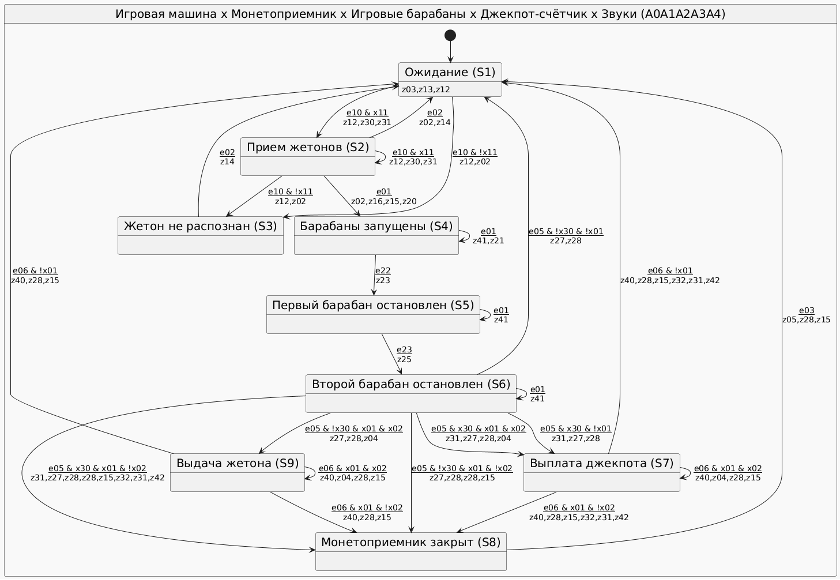
\includegraphics[width=0.8\linewidth]{media/image3.png}\end{center}
% @p 176
Рис. 6. Диаграмма состояний итогового автомата $A_{0}$*$A_{1}$*$A_{2}$*$A_{3}$*$A_{4}$ (9 состояний). Состояния подписаны сокращёнными названиями; соответствие каждого состояния исходным состояниям пяти автоматов приведено ниже

% @p 177
S1 – $A_{0}$: Ожидание, $A_{1}$: Монетоприемник пуст, $A_{2}$: Барабаны остановлены, $A_{3}$: Накопление, $A_{4}$: Ожидание

% @p 178
S2 – $A_{0}$: Прием жетонов, $A_{1}$: Жетон принят, $A_{2}$: Барабаны остановлены, $A_{3}$: Накопление, $A_{4}$: Ожидание

% @p 179
S3 – $A_{0}$: Ошибка, $A_{1}$: Жетон не распознан, $A_{2}$: Барабаны остановлены, $A_{3}$: Накопление, $A_{4}$: Ожидание

% @p 180
S4 – $A_{0}$: Игра, $A_{1}$: Монетоприемник закрыт, $A_{2}$: Барабаны запущены, $A_{3}$: Накопление, $A_{4}$: Ожидание

% @p 181
S5 – $A_{0}$: Игра, $A_{1}$: Монетоприемник закрыт, $A_{2}$: Первый барабан остановлен, $A_{3}$: Накопление, $A_{4}$: Ожидание

% @p 182
S6 – $A_{0}$: Игра, $A_{1}$: Монетоприемник закрыт, $A_{2}$: Второй барабан остановлен, $A_{3}$: Накопление, $A_{4}$: Ожидание

% @p 183
S7 – $A_{0}$: Выдача жетона, $A_{1}$: Монетоприемник закрыт, $A_{2}$: Барабаны остановлены, $A_{3}$: Выплата джекпота, $A_{4}$: Ожидание

% @p 184
S8 – $A_{0}$: Ошибка, $A_{1}$: Монетоприемник закрыт, $A_{2}$: Барабаны остановлены, $A_{3}$: Накопление, $A_{4}$: Ожидание

% @p 185
S9 – $A_{0}$: Выдача жетона, $A_{1}$: Монетоприемник закрыт, $A_{2}$: Барабаны остановлены, $A_{3}$: Накопление, $A_{4}$: Ожидание

% @p 186
Таблица 7. Входные и выходные воздействия автомата «Игровая машина * Монетоприемник * Игровые барабаны * Джекпот-счётчик * Звуки» (A0A1A2A3A4)

% @img 187
\begin{center}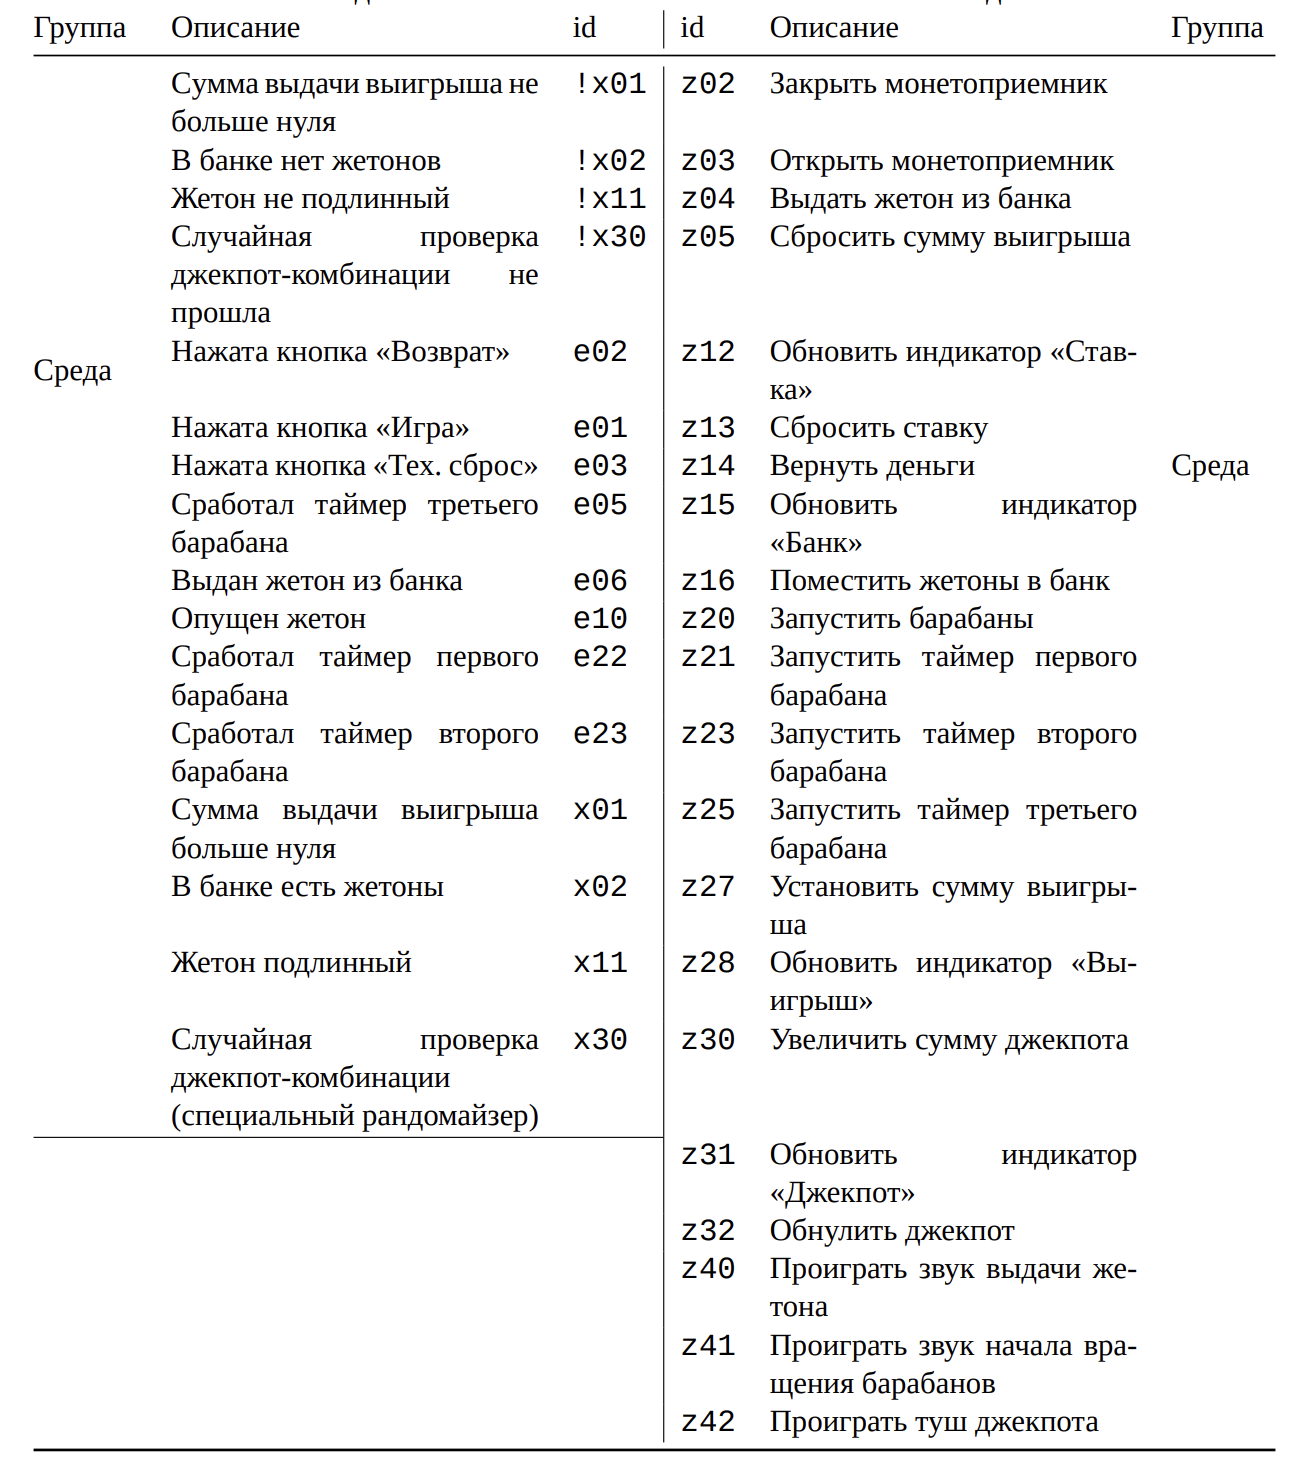
\includegraphics[width=0.8\linewidth]{media/image9.png}\end{center}
% @p 190
\subsection*{Вывод}

% @p 191
% 1 итог; 2 связь: раскрывает итог по ограничениям; 3 связь: «вместе это» – общее следствие;
% 4 связь: «кроме того» – результаты сверх ограничений.
Предложенные доработки снимают три ограничения предыдущей работы. Теперь в состояние можно вложить несколько автоматов (ограничение 1), автомат можно вложить в несколько состояний (ограничение 2), а вложенные автоматы могут содержать оба перемножаемых автомата (ограничение 3). Вместе это позволяет строить цепочки вложенности любой глубины. Кроме того, исправлена ошибка, при которой вложенный автомат реагировал на адресованное событие отдельно от перехода отправителя (доработка 3), и адресованное событие теперь получают также автоматы, вложенные в состояние получателя (доработка 4).

% @p 192
% 1 тезис; 2, 3 связь: два случая из тезиса; 4 связь: где порядок не важен.
Порядок перемножения автоматов по-прежнему важен в двух случаях. Автомат, на состояние которого ссылается гвард, должен войти в произведение не позднее автомата с этим гвардом. Автомат, который получает адресованные события через вложенность, должен войти в произведение после родительского. Для адресованных событий, которые приходят напрямую, порядок не важен.

% @p 193
% 1 результат; 2 связь: с чем сравнить; 3 связь: что результат правильный; 4 связь: где взять программу.
Для системы из пяти автоматов итоговое произведение содержит девять состояний. В исходной системе 16 состояний, а верхняя оценка числа состояний произведения равна 5·4·4·2·1 = 160. Автомат-произведение и исходная система функционируют одинаково на всех последовательностях входных воздействий длиной до 20 и на 1000 случайных последовательностях длиной 100. Программа, которая реализует предлагаемый метод перемножения автоматов, опубликована по адресу https://github.com/PhoenixNazarov/fsm-multiply.

\end{document}
